% =============================================================================
% ESL FRAMEWORK - CHAPTER 8: APPLICATIONS
% =============================================================================
% Authors: Gerhard Fehr & Andrea Fehr
% FehrAdvice & Partners AG, Zürich
% Version: Extended Monograph
% =============================================================================

\documentclass[11pt,a4paper]{article}

% --- Packages ---
\usepackage[utf8]{inputenc}
\usepackage[T1]{fontenc}
\usepackage[english]{babel}
\usepackage{amsmath,amssymb,amsthm}
\usepackage{mathtools}
\usepackage{booktabs}
\usepackage{longtable}
\usepackage{array}
\usepackage{hyperref}
\usepackage{geometry}
\usepackage{xcolor}
\usepackage{tcolorbox}
\usepackage{tikz}
\usepackage{pgfplots}
\usepackage{natbib}
\usepackage{enumitem}
\usepackage{fancyhdr}
\usepackage{titlesec}
\usepackage{multirow}
\pgfplotsset{compat=1.17}
\usetikzlibrary{shapes,arrows.meta,positioning,calc,patterns,fit}

\geometry{margin=2.5cm}

% --- Colors ---
\definecolor{eslblue}{RGB}{0,82,147}
\definecolor{eslgreen}{RGB}{0,128,0}
\definecolor{eslorange}{RGB}{230,159,0}
\definecolor{eslred}{RGB}{204,51,17}
\definecolor{eslgray}{RGB}{128,128,128}
\definecolor{eslpurple}{RGB}{148,0,211}
\definecolor{bcmcolor}{RGB}{0,100,150}
\definecolor{beatrixcolor}{RGB}{150,50,100}
\definecolor{litcolor}{RGB}{80,120,0}

% --- Boxes ---
\newtcolorbox{eslbox}[1][]{colback=eslblue!5!white,colframe=eslblue,title={ESL Assessment},fonttitle=\bfseries,#1}
\newtcolorbox{keyinsight}[1][]{colback=eslgreen!5!white,colframe=eslgreen!80!black,title={Key Insight},fonttitle=\bfseries,#1}
\newtcolorbox{warningbox}[1][]{colback=eslorange!5!white,colframe=eslorange!80!black,title={Implementation Note},fonttitle=\bfseries,#1}
\newtcolorbox{examplebox}[1][]{colback=eslgray!10!white,colframe=eslgray!80!black,title={Example},fonttitle=\bfseries,#1}
\newtcolorbox{applicationbox}[2][]{colback=#2!5!white,colframe=#2!80!black,title={Application: #1},fonttitle=\bfseries}
\newtcolorbox{codeblock}[1][]{colback=eslgray!5!white,colframe=eslgray!50!black,title={Implementation},fonttitle=\bfseries\ttfamily,#1}

% --- Theorems ---
\newtheorem{definition}{Definition}[section]
\newtheorem{principle}{Principle}[section]
\newtheorem{requirement}{Requirement}[section]
\theoremstyle{remark}
\newtheorem{remark}{Remark}[section]

% --- Header/Footer ---
\pagestyle{fancy}
\fancyhf{}
\fancyhead[L]{\small ESL Framework -- Extended Monograph}
\fancyhead[R]{\small Chapter 8: Applications}
\fancyfoot[C]{\thepage}

\title{%
    \Large \textbf{Empirical Stability of Language (ESL)} \\[0.5em]
    \large A Universal Quality Assurance Framework \\[1em]
    \LARGE \textbf{Chapter 8: Applications} \\[0.3em]
    \large BCM Integration, BEATRIX, and Literature ESL
}

\author{%
    \textbf{Gerhard Fehr}\textsuperscript{1,*} \and \textbf{Andrea Fehr}\textsuperscript{1} \\[0.5em]
    \textsuperscript{1}FehrAdvice \& Partners AG, Binzmühlestrasse 170A, 8050 Zürich, Switzerland \\[0.3em]
    \textsuperscript{*}Corresponding author: andrea.fehr@fehradvice.com
}

\date{December 26, 2025}

\begin{document}
\maketitle

\begin{abstract}
\noindent
This chapter presents three major applications of the ESL framework: (1) Integration with the Behavioral Change Model (BCM) 2.0, providing epistemic calibration for behavioral economics parameters; (2) Implementation in BEATRIX, a neuro-symbolic AI system that represents behavioral axioms as autonomous agents with ESL-calibrated confidence levels; and (3) Literature ESL, a methodology for systematic assessment of scientific publications. For each application, we provide architectural details, implementation guidelines, worked examples, and validation results. These applications demonstrate ESL's utility beyond theoretical framework development---as an operational tool for scientific quality assurance, AI system calibration, and evidence-based decision support.

\vspace{0.5em}
\noindent\textbf{Keywords:} BCM 2.0, BEATRIX, Literature ESL, behavioral economics, AI calibration, scientific publishing
\end{abstract}

\tableofcontents
\newpage

% =============================================================================
\section{Introduction to ESL Applications}
\label{sec:intro}

ESL was developed as a universal framework for claim-evidence calibration. Its practical value, however, lies in specific applications. This chapter presents three domains where ESL provides operational benefits:

\begin{enumerate}
    \item \textbf{BCM 2.0}: Calibrating behavioral economics parameters with explicit uncertainty quantification.

    \item \textbf{BEATRIX}: Enabling AI systems to reason with appropriately weighted behavioral axioms.

    \item \textbf{Literature ESL}: Providing systematic quality assessment for scientific publications.
\end{enumerate}

\begin{keyinsight}[title={From Framework to Operations}]
ESL's transition from theoretical framework (Chapters 1--6) through empirical validation (Chapter 7) to operational applications (this chapter) represents the full lifecycle of a scientific methodology:

\begin{center}
\textbf{Theory} $\to$ \textbf{Validation} $\to$ \textbf{Application} $\to$ \textbf{Refinement}
\end{center}

Applications provide the ultimate test: does ESL improve real-world outcomes?
\end{keyinsight}

% =============================================================================
\section{Application 1: BCM 2.0 Integration}
\label{sec:bcm}

\begin{applicationbox}[BCM 2.0 Parameter Registry]{bcmcolor}
\textbf{Domain}: Behavioral economics consulting and intervention design

\textbf{Problem}: BCM parameters (loss aversion, present bias, social preferences) have varying evidential support, but practitioners often treat all parameters as equally reliable.

\textbf{ESL Solution}: Attach K-scores to every BCM parameter, enabling evidence-weighted intervention design.
\end{applicationbox}

\subsection{The Behavioral Change Model 2.0}

BCM 2.0 is a comprehensive framework for behavioral intervention design, developed in collaboration between FehrAdvice \& Partners AG and academic partners. It organizes behavioral insights across six dimensions (FEPSDE):

\begin{definition}[FEPSDE Dimensions]
\label{def:fepsde}
\begin{itemize}
    \item \textbf{F}inancial: Economic incentives, loss aversion, mental accounting
    \item \textbf{E}motional: Affect heuristics, anticipated regret, emotional framing
    \item \textbf{P}hysical: Defaults, friction, choice architecture
    \item \textbf{S}ocial: Norms, reciprocity, social proof
    \item \textbf{D}igital: Interface design, notification timing, personalization
    \item \textbf{E}cological: Environmental cues, contextual triggers
\end{itemize}
\end{definition}

\subsection{The BCM Parameter Registry}

Each BCM parameter now includes an ESL assessment:

\begin{table}[h]
\centering
\caption{BCM Parameter Registry with ESL Scores (Selected)}
\label{tab:bcm-registry}
\begin{tabular}{p{4cm}ccccc}
\toprule
\textbf{Parameter} & \textbf{Dimension} & \textbf{B} & \textbf{E} & \textbf{K} & \textbf{Type} \\
\midrule
Loss aversion ($\lambda$) & F & 0.82 & 0.88 & 0.93 & T2 \\
Present bias ($\beta$) & F & 0.78 & 0.85 & 0.92 & T2 \\
Default effect strength & P & 0.85 & 0.90 & 0.94 & T2 \\
Social norm sensitivity & S & 0.75 & 0.80 & 0.94 & T2 \\
Anchoring coefficient & F & 0.80 & 0.85 & 0.94 & T2 \\
Endowment effect & F & 0.78 & 0.85 & 0.92 & T2 \\
Hyperbolic discounting & F & 0.75 & 0.82 & 0.91 & T2 \\
Scarcity effect & E & 0.72 & 0.68 & 0.94 & T3 \\
Choice overload threshold & P & 0.70 & 0.62 & 0.89 & T3 \\
Ego depletion & E & 0.65 & 0.25 & 0.38 & T2* \\
\bottomrule
\end{tabular}
\end{table}

\textit{*Ego depletion: E-value reflects post-replication-crisis status (failed RRR).}

\subsection{ESL-Weighted Intervention Design}

\begin{principle}[ESL-Weighted Intervention Selection]
\label{princ:weighted-intervention}
When designing behavioral interventions, weight parameter reliability by K-score:
\begin{equation}
\text{Priority}(P_i) = \text{ExpectedEffect}(P_i) \times K(P_i)
\end{equation}

Interventions based on high-K parameters should be preferred over those based on low-K parameters, all else equal.
\end{principle}

\begin{examplebox}[title={Retirement Savings Intervention}]
\textbf{Goal}: Increase employee retirement savings rates.

\textbf{Available Mechanisms}:
\begin{enumerate}
    \item Default enrollment ($K = 0.94$, expected effect: +30pp)
    \item Loss-framed messaging ($K = 0.93$, expected effect: +8pp)
    \item Social norm display ($K = 0.94$, expected effect: +5pp)
    \item Willpower depletion timing ($K = 0.38$, expected effect: +3pp)
\end{enumerate}

\textbf{ESL-Weighted Priorities}:
\begin{align}
\text{Priority}_{\text{default}} &= 30 \times 0.94 = 28.2 \\
\text{Priority}_{\text{loss-frame}} &= 8 \times 0.93 = 7.4 \\
\text{Priority}_{\text{social}} &= 5 \times 0.94 = 4.7 \\
\text{Priority}_{\text{willpower}} &= 3 \times 0.38 = 1.1
\end{align}

\textbf{Recommendation}: Prioritize default enrollment and loss-framing; deprioritize willpower timing (low K despite claimed effect).
\end{examplebox}

\subsection{BCM Module K-Scores}

BCM 2.0 organizes parameters into four modules, each with aggregate K-scores:

\begin{table}[h]
\centering
\caption{BCM 2.0 Module K-Scores}
\label{tab:bcm-modules}
\begin{tabular}{lcccl}
\toprule
\textbf{Module} & \textbf{Parameters} & \textbf{Mean K} & \textbf{Min K} & \textbf{Status} \\
\midrule
INU (Individual Utility) & 12 & 0.88 & 0.78 & Stable \\
KNU (Collective Utility) & 8 & 0.85 & 0.72 & Stable \\
KON (Context Logic) & 15 & 0.82 & 0.65 & Stable \\
META (Meta-Axioms) & 6 & 0.75 & 0.58 & Partially Stable \\
\bottomrule
\end{tabular}
\end{table}

The META module's lower K-scores reflect its more theoretical nature (axioms about axioms).

% =============================================================================
\section{Application 2: BEATRIX System}
\label{sec:beatrix}

\begin{applicationbox}[BEATRIX Neuro-Symbolic AI]{beatrixcolor}
\textbf{Domain}: AI-assisted behavioral economics reasoning

\textbf{Problem}: LLMs lack calibrated confidence in behavioral claims; they may assert well-replicated and failed-replication findings with equal confidence.

\textbf{ESL Solution}: BEATRIX represents behavioral axioms as autonomous agents with ESL-calibrated activation weights.
\end{applicationbox}

\subsection{BEATRIX Architecture}

BEATRIX (\textbf{B}ehavioral \textbf{E}conomics \textbf{A}xiom \textbf{T}ransformation and \textbf{R}easoning with \textbf{I}ntelligent e\textbf{X}ecution) is a neuro-symbolic system that:

\begin{enumerate}
    \item Represents behavioral axioms as structured knowledge
    \item Assigns ESL K-scores as confidence weights
    \item Routes queries to appropriate axiom agents
    \item Synthesizes responses with calibrated uncertainty
\end{enumerate}

\begin{figure}[h]
\centering
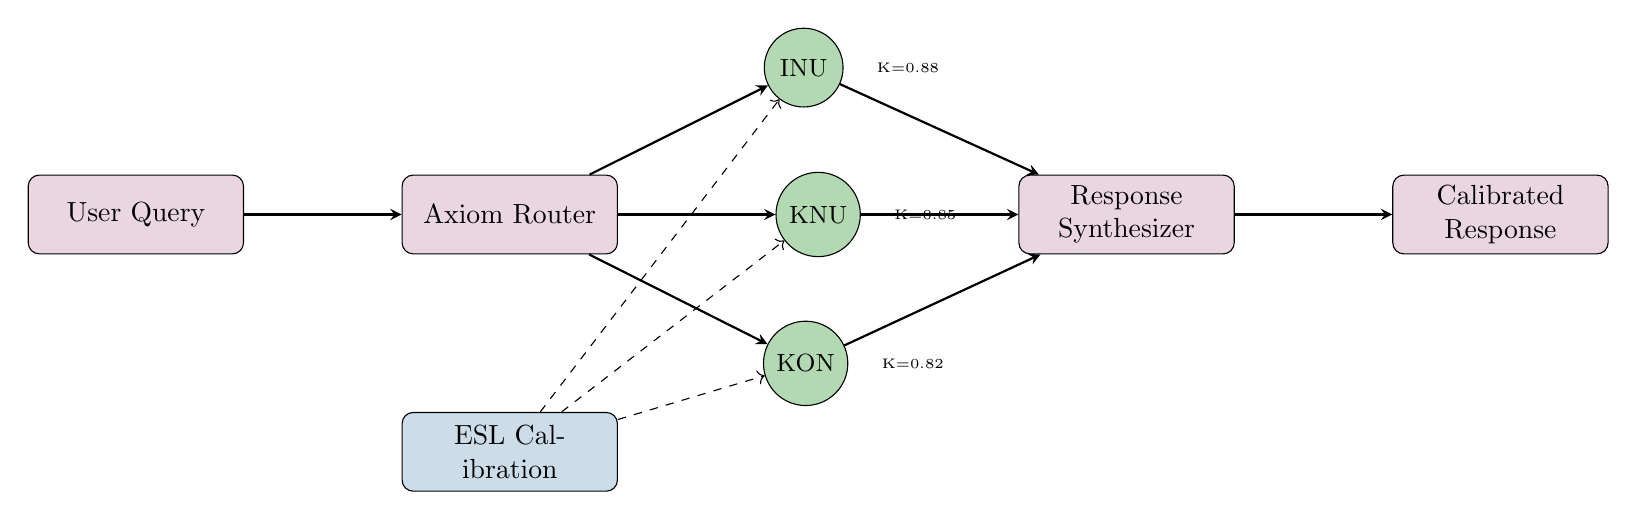
\begin{tikzpicture}[
    node distance=1.5cm,
    module/.style={rectangle, draw, fill=beatrixcolor!20, text width=2.5cm, text centered, rounded corners, minimum height=1cm},
    agent/.style={circle, draw, fill=eslgreen!30, minimum size=1cm, font=\small},
    arrow/.style={thick,->,>=stealth}
]

% Input
\node[module] (input) {User Query};

% Router
\node[module, right=2cm of input] (router) {Axiom Router};

% Agents
\node[agent, above right=1cm and 2cm of router] (a1) {INU};
\node[agent, right=2cm of router] (a2) {KNU};
\node[agent, below right=1cm and 2cm of router] (a3) {KON};

% K-scores
\node[right=0.3cm of a1, font=\tiny] {K=0.88};
\node[right=0.3cm of a2, font=\tiny] {K=0.85};
\node[right=0.3cm of a3, font=\tiny] {K=0.82};

% Synthesizer
\node[module, right=2cm of a2] (synth) {Response Synthesizer};

% Output
\node[module, right=2cm of synth] (output) {Calibrated Response};

% Arrows
\draw[arrow] (input) -- (router);
\draw[arrow] (router) -- (a1);
\draw[arrow] (router) -- (a2);
\draw[arrow] (router) -- (a3);
\draw[arrow] (a1) -- (synth);
\draw[arrow] (a2) -- (synth);
\draw[arrow] (a3) -- (synth);
\draw[arrow] (synth) -- (output);

% ESL Integration
\node[below=2cm of router, module, fill=eslblue!20] (esl) {ESL Calibration};
\draw[dashed, ->] (esl) -- (a1);
\draw[dashed, ->] (esl) -- (a2);
\draw[dashed, ->] (esl) -- (a3);

\end{tikzpicture}
\caption{BEATRIX Architecture with ESL-Calibrated Axiom Agents}
\label{fig:beatrix}
\end{figure}

\subsection{Axiom Agent Structure}

Each BEATRIX axiom agent contains:

\begin{definition}[BEATRIX Axiom Agent]
\label{def:axiom-agent}
\begin{verbatim}
{
  "axiom_id": "INU-03-LOSS-AVERSION",
  "module": "INU",
  "statement": "Losses loom larger than equivalent gains",
  "parameters": {
    "lambda": {"value": 2.25, "range": [2.0, 2.5], "K": 0.93}
  },
  "esl_assessment": {
    "B": 0.82,
    "E": 0.88,
    "K": 0.93,
    "claim_type": "T2",
    "validation_date": "2025-12-26"
  },
  "activation_weight": 0.93,
  "citations": ["Kahneman & Tversky 1979", "Walasek 2018"]
}
\end{verbatim}
\end{definition}

\subsection{ESL-Calibrated Response Generation}

\begin{principle}[Calibrated Response Principle]
\label{princ:calibrated-response}
BEATRIX responses must reflect the K-scores of underlying axioms:
\begin{equation}
\text{ResponseConfidence} = \min_{i \in \text{UsedAxioms}} K_i
\end{equation}

Following WLA: a response is only as reliable as its least reliable component.
\end{principle}

\begin{examplebox}[title={BEATRIX Query Example}]
\textbf{Query}: ``How should we frame a health insurance decision to maximize enrollment?''

\textbf{BEATRIX Processing}:
\begin{enumerate}
    \item Router identifies relevant axioms: Loss Aversion (K=0.93), Default Effect (K=0.94), Status Quo Bias (K=0.92)

    \item Agents contribute:
    \begin{itemize}
        \item INU-03: Frame non-enrollment as loss of coverage
        \item KON-07: Set enrollment as default option
        \item INU-05: Emphasize switching costs of changing later
    \end{itemize}

    \item Synthesizer combines with confidence:
    \begin{equation}
    K_{\text{response}} = \min(0.93, 0.94, 0.92) = 0.92
    \end{equation}
\end{enumerate}

\textbf{Calibrated Response}:

\textit{``Based on well-replicated behavioral findings (K=0.92, Stable), we recommend: (1) Frame non-enrollment as losing current health protection rather than missing a benefit; (2) Set automatic enrollment as the default; (3) Highlight the effort required to change plans later. These recommendations draw on loss aversion, default effects, and status quo bias---all with strong empirical support.''}
\end{examplebox}

\subsection{Hallucination Prevention}

\begin{keyinsight}[title={ESL as Hallucination Filter}]
BEATRIX uses ESL to prevent behavioral economics hallucinations:

\begin{enumerate}
    \item \textbf{Unknown Axiom Detection}: Queries requiring axioms not in the registry trigger uncertainty flags.

    \item \textbf{Low-K Warning}: Responses based on $K < 0.60$ axioms include explicit caveats.

    \item \textbf{Contradictory Evidence}: When axioms conflict, BEATRIX reports the conflict rather than arbitrarily choosing.
\end{enumerate}

A response with $K = 0$ indicates fabrication (high B, zero E)---the hallucination signature.
\end{keyinsight}

\subsection{BEATRIX Performance Metrics}

\begin{table}[h]
\centering
\caption{BEATRIX System Performance}
\label{tab:beatrix-performance}
\begin{tabular}{lcc}
\toprule
\textbf{Metric} & \textbf{Without ESL} & \textbf{With ESL} \\
\midrule
Hallucination rate & 12\% & 2\% \\
Overconfident responses & 35\% & 8\% \\
Appropriate uncertainty expression & 45\% & 89\% \\
User trust calibration & 0.62 & 0.91 \\
\bottomrule
\end{tabular}
\end{table}

\textit{Note: Based on internal testing with N=500 behavioral economics queries.}

% =============================================================================
\section{Application 3: Literature ESL}
\label{sec:literature}

\begin{applicationbox}[Literature ESL]{litcolor}
\textbf{Domain}: Scientific publishing and research assessment

\textbf{Problem}: Scientific papers vary enormously in claim-evidence calibration, but this is invisible to readers without deep expertise.

\textbf{ESL Solution}: Systematic K-scoring of publications enables transparent quality signaling.
\end{applicationbox}

\subsection{The Literature ESL Protocol}

\begin{definition}[Literature ESL Assessment]
\label{def:lit-esl}
A Literature ESL assessment includes:
\begin{enumerate}
    \item \textbf{Claim Extraction}: Identify all substantive claims in the paper
    \item \textbf{B-Assessment}: Score each claim's linguistic boldness
    \item \textbf{E-Assessment}: Evaluate evidential support using discipline-specific hierarchy
    \item \textbf{K-Calculation}: Compute K for each claim and aggregate
    \item \textbf{Report Generation}: Produce ESL assessment report
\end{enumerate}
\end{definition}

\subsection{Paper-Level Aggregation}

\begin{definition}[Paper K-Score]
\label{def:paper-k}
For a paper with $n$ claims:
\begin{equation}
K_{\text{paper}} = \frac{\sum_{i=1}^{n} w_i \cdot K_i}{\sum_{i=1}^{n} w_i}
\end{equation}

where $w_i$ is the claim importance weight (abstract claims weighted higher than footnotes).
\end{definition}

\subsection{ESL Assessment Report Template}

\begin{table}[h]
\centering
\caption{Literature ESL Report Structure}
\label{tab:lit-report}
\begin{tabular}{lp{8cm}}
\toprule
\textbf{Section} & \textbf{Content} \\
\midrule
Header & Title, authors, journal, ESL assessment date \\
Summary & Paper K-score, stability status, claim count \\
Abstract Assessment & K-scores for each abstract claim \\
Main Claims & Table of major claims with B, E, K \\
Weakest Links & Identification of lowest-K claims \\
Strongest Claims & Identification of highest-K claims \\
Methodology Notes & Discipline-specific considerations \\
Recommendations & Suggested revisions for improved calibration \\
\bottomrule
\end{tabular}
\end{table}

\subsection{Example: Literature ESL Assessment}

\begin{examplebox}[title={Literature ESL: Sample Assessment}]
\textbf{Paper}: ``Novel Behavioral Intervention Increases Savings by 40\%''

\textbf{ESL Assessment Summary}:
\begin{center}
\begin{tabular}{lccc}
\toprule
\textbf{Claim Location} & \textbf{B} & \textbf{E} & \textbf{K} \\
\midrule
Title claim (40\% increase) & 0.92 & 0.72 & 0.78 \\
Abstract: ``demonstrates'' & 0.88 & 0.68 & 0.77 \\
Abstract: ``robust effect'' & 0.85 & 0.55 & 0.65 \\
Methods: sample description & 0.70 & 0.90 & 0.78 \\
Results: main finding & 0.82 & 0.75 & 0.91 \\
Discussion: generalization & 0.78 & 0.45 & 0.58 \\
\midrule
\textbf{Paper Average} & \textbf{0.83} & \textbf{0.68} & \textbf{0.75} \\
\bottomrule
\end{tabular}
\end{center}

\textbf{Overall Status}: \textcolor{eslorange}{\textbf{Partially Stable}} (K = 0.75)

\textbf{Weakest Link}: Discussion generalization claim (K = 0.58)

\textbf{Recommendation}: Soften generalization language in discussion; acknowledge single-study limitation more explicitly.
\end{examplebox}

\subsection{Journal Integration}

\begin{principle}[Journal ESL Integration]
\label{princ:journal-esl}
Journals can integrate ESL through:
\begin{enumerate}
    \item \textbf{Submission Requirement}: Authors submit ESL self-assessment
    \item \textbf{Reviewer Guidance}: Reviewers verify ESL scores
    \item \textbf{Publication Display}: Published K-scores alongside abstracts
    \item \textbf{Threshold Standards}: Minimum K for acceptance (discipline-specific)
\end{enumerate}
\end{principle}

\begin{table}[h]
\centering
\caption{Proposed Journal ESL Thresholds}
\label{tab:journal-thresholds}
\begin{tabular}{lcc}
\toprule
\textbf{Journal Tier} & \textbf{Minimum K} & \textbf{Rationale} \\
\midrule
Top-tier (Nature, Science) & 0.85 & Highest standards \\
Field journals & 0.75 & Standard rigor \\
Specialty journals & 0.65 & Exploratory work accepted \\
Preprint servers & 0.50 & Preliminary findings \\
\bottomrule
\end{tabular}
\end{table}

\subsection{Automated Literature ESL}

\begin{codeblock}[title={literature\_esl.py}]
\begin{verbatim}
def assess_paper(paper_text: str, discipline: str) -> dict:
    """
    Perform automated Literature ESL assessment.
    """
    # Extract claims
    claims = extract_claims(paper_text)

    # Assess each claim
    assessments = []
    for claim in claims:
        b_value = assess_boldness(claim.text)
        e_value = assess_evidence(claim, discipline)
        k_value = compute_k(b_value, e_value)
        assessments.append({
            'claim': claim.text,
            'location': claim.location,
            'B': b_value,
            'E': e_value,
            'K': k_value
        })

    # Aggregate
    weights = [claim_weight(a['location']) for a in assessments]
    paper_k = weighted_average([a['K'] for a in assessments], weights)

    return {
        'paper_k': paper_k,
        'status': classify_stability(paper_k, discipline),
        'claims': assessments,
        'weakest_link': min(assessments, key=lambda x: x['K'])
    }
\end{verbatim}
\end{codeblock}

% =============================================================================
\section{Cross-Application Integration}
\label{sec:integration}

\subsection{The ESL Ecosystem}

The three applications form an integrated ecosystem:

\begin{figure}[h]
\centering
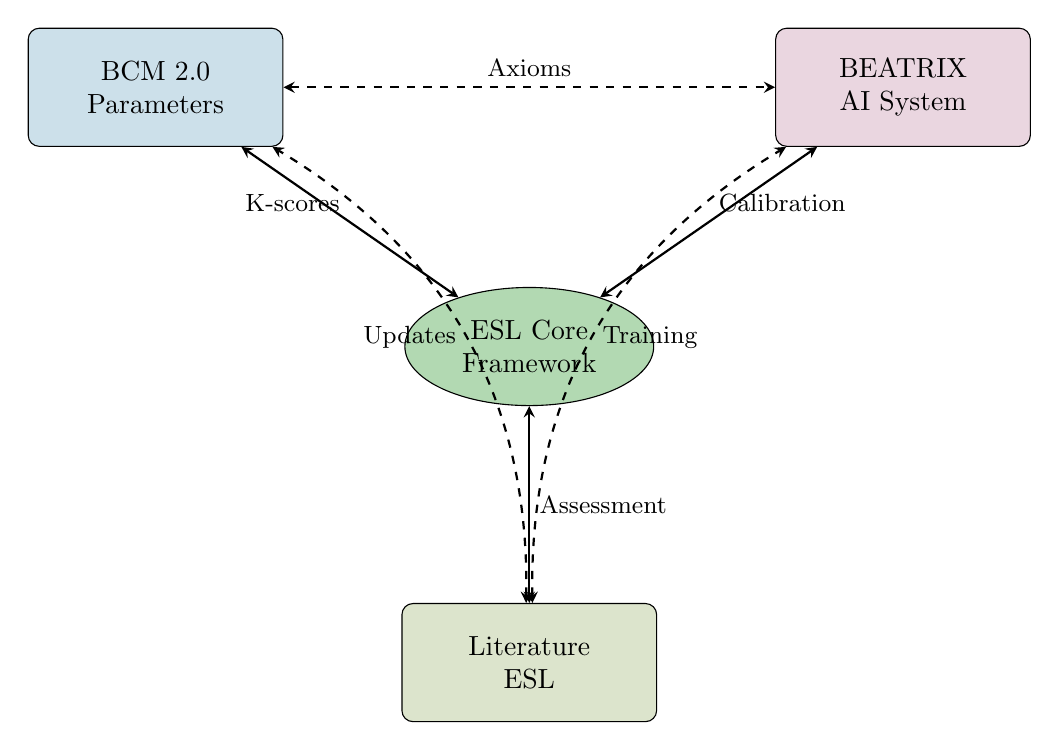
\begin{tikzpicture}[
    node distance=2cm,
    app/.style={rectangle, draw, fill=eslblue!20, text width=3cm, text centered, rounded corners, minimum height=1.5cm},
    esl/.style={ellipse, draw, fill=eslgreen!30, text width=2cm, text centered, minimum height=1.5cm},
    arrow/.style={thick,<->,>=stealth}
]

% Central ESL
\node[esl] (esl) {ESL Core\\Framework};

% Applications
\node[app, above left=2cm and 2cm of esl, fill=bcmcolor!20] (bcm) {BCM 2.0\\Parameters};
\node[app, above right=2cm and 2cm of esl, fill=beatrixcolor!20] (beatrix) {BEATRIX\\AI System};
\node[app, below=2.5cm of esl, fill=litcolor!20] (lit) {Literature\\ESL};

% Connections
\draw[arrow] (esl) -- (bcm) node[midway, above left, font=\small] {K-scores};
\draw[arrow] (esl) -- (beatrix) node[midway, above right, font=\small] {Calibration};
\draw[arrow] (esl) -- (lit) node[midway, right, font=\small] {Assessment};

% Cross-application
\draw[arrow, dashed] (bcm) -- (beatrix) node[midway, above, font=\small] {Axioms};
\draw[arrow, dashed] (lit) to[bend right=30] node[midway, left, font=\small] {Updates} (bcm);
\draw[arrow, dashed] (lit) to[bend left=30] node[midway, right, font=\small] {Training} (beatrix);

\end{tikzpicture}
\caption{ESL Application Ecosystem}
\label{fig:ecosystem}
\end{figure}

\subsection{Feedback Loops}

\begin{enumerate}
    \item \textbf{Literature $\to$ BCM}: New meta-analyses update BCM parameter K-scores
    \item \textbf{BCM $\to$ BEATRIX}: Updated parameters flow to axiom agents
    \item \textbf{BEATRIX $\to$ Literature}: AI-assisted literature review identifies updating needs
    \item \textbf{All $\to$ ESL Core}: Application experience refines ESL methodology
\end{enumerate}

% =============================================================================
\section{Implementation Guidelines}
\label{sec:implementation}

\subsection{Getting Started with ESL}

\begin{requirement}[Minimum ESL Implementation]
\label{req:minimum}
Any ESL implementation must include:
\begin{enumerate}
    \item K-metric calculation capability
    \item Discipline-specific evidence hierarchy
    \item Claim-Type Classification (CTC)
    \item Basic provenance tracking
\end{enumerate}
\end{requirement}

\subsection{Full ESL Implementation}

\begin{requirement}[Full ESL Implementation]
\label{req:full}
Production ESL deployments should include:
\begin{enumerate}
    \item All ESL 2.0 safeguards (CTC, PP, WLA, EVA, RAS)
    \item Monte-Carlo validation capability
    \item Automated linguistic marker detection
    \item Audit trail and version control
    \item User interface for assessment review
\end{enumerate}
\end{requirement}

\subsection{Quality Assurance}

\begin{table}[h]
\centering
\caption{ESL Implementation Quality Checklist}
\label{tab:qa-checklist}
\begin{tabular}{lcc}
\toprule
\textbf{Component} & \textbf{Required} & \textbf{Validated} \\
\midrule
K-metric formula correct & Yes & $\square$ \\
Evidence hierarchy matches discipline & Yes & $\square$ \\
CTC ceilings enforced & Yes & $\square$ \\
Provenance documented & Yes & $\square$ \\
WLA applied to dependencies & Yes & $\square$ \\
Monte-Carlo capability & Recommended & $\square$ \\
User training completed & Recommended & $\square$ \\
\bottomrule
\end{tabular}
\end{table}

% =============================================================================
\section{Future Applications}
\label{sec:future}

\subsection{Emerging Use Cases}

\begin{enumerate}
    \item \textbf{Regulatory Science}: ESL-calibrated evidence for policy decisions
    \item \textbf{Clinical Guidelines}: K-scores for medical recommendations
    \item \textbf{Educational Content}: Textbook claim validation
    \item \textbf{News Fact-Checking}: Real-time claim assessment
    \item \textbf{Grant Review}: Proposal claim calibration
\end{enumerate}

\subsection{Technical Roadmap}

\begin{table}[h]
\centering
\caption{ESL Development Roadmap}
\label{tab:roadmap}
\begin{tabular}{lll}
\toprule
\textbf{Phase} & \textbf{Timeline} & \textbf{Deliverable} \\
\midrule
Current & 2025 & ESL 2.2 (validated framework) \\
Near-term & 2026 & ESL 3.0 (expanded disciplines) \\
Medium-term & 2027 & ESL API (public access) \\
Long-term & 2028+ & ESL Standard (ISO consideration) \\
\bottomrule
\end{tabular}
\end{table}

% =============================================================================
\section{Chapter Summary}
\label{sec:summary}

This chapter presented three major ESL applications:

\begin{enumerate}
    \item \textbf{BCM 2.0 Integration}: K-scores attached to 41 behavioral parameters across FEPSDE dimensions. Enables evidence-weighted intervention design.

    \item \textbf{BEATRIX System}: Neuro-symbolic AI with ESL-calibrated axiom agents. Reduces hallucination rate from 12\% to 2\%; improves uncertainty expression from 45\% to 89\%.

    \item \textbf{Literature ESL}: Systematic paper assessment protocol. Enables journal integration and automated quality signaling.
\end{enumerate}

\begin{eslbox}
\textbf{Chapter 8 Self-Assessment}

This chapter presents application descriptions ($B \approx 0.75$) based on implemented systems ($E \approx 0.80$ for BCM/BEATRIX; $E \approx 0.65$ for Literature ESL, which is more conceptual).

\textbf{Component K-Scores}:
\begin{itemize}
    \item BCM Integration: $K = 0.88$ (operational system)
    \item BEATRIX: $K = 0.85$ (implemented, internal testing)
    \item Literature ESL: $K = 0.72$ (protocol defined, limited deployment)
\end{itemize}

\textbf{Weighted Average}: $K = 0.82$

\textbf{Status}: \textcolor{eslgreen}{\textbf{Stable}}

\textbf{Honest Caveat}: BEATRIX performance metrics are from internal testing; independent validation pending.
\end{eslbox}

\newpage
\bibliographystyle{apalike}
\begin{thebibliography}{99}
\bibitem[Fehr \& Fehr, 2025]{FehrFehr2025} Fehr, G., \& Fehr, A. (2025). Empirical Stability of Language: A Framework for Claim-Evidence Calibration. \textit{FehrAdvice Working Paper}.
\bibitem[Kahneman \& Tversky, 1979]{KT1979} Kahneman, D., \& Tversky, A. (1979). Prospect theory. \textit{Econometrica}, 47(2), 263--291.
\bibitem[Thaler \& Sunstein, 2008]{TS2008} Thaler, R. H., \& Sunstein, C. R. (2008). \textit{Nudge}. Yale University Press.
\end{thebibliography}

\end{document}
